\subsection{Pipelined Design}
So what is the purpose of a Pipelined version of a CPU\@? As stated in the previous section, the unpipelined version is quite slow since it needs to wait for the instruction to be executed before loading the next one. 
Pipelining follows the idea of dividing the work among smaller parts and executing them in parallel. In the case of a CPU, it means that we will divide the execution of an instruction into multiple stages and execute multiple instructions at the same time.
Since each part has a smaller quantity of work to do, we can hopefully increase the clock frequency and thus obtaining in average a better throughput resulting in better performance.

\begin{figure}[H]
    \centering
    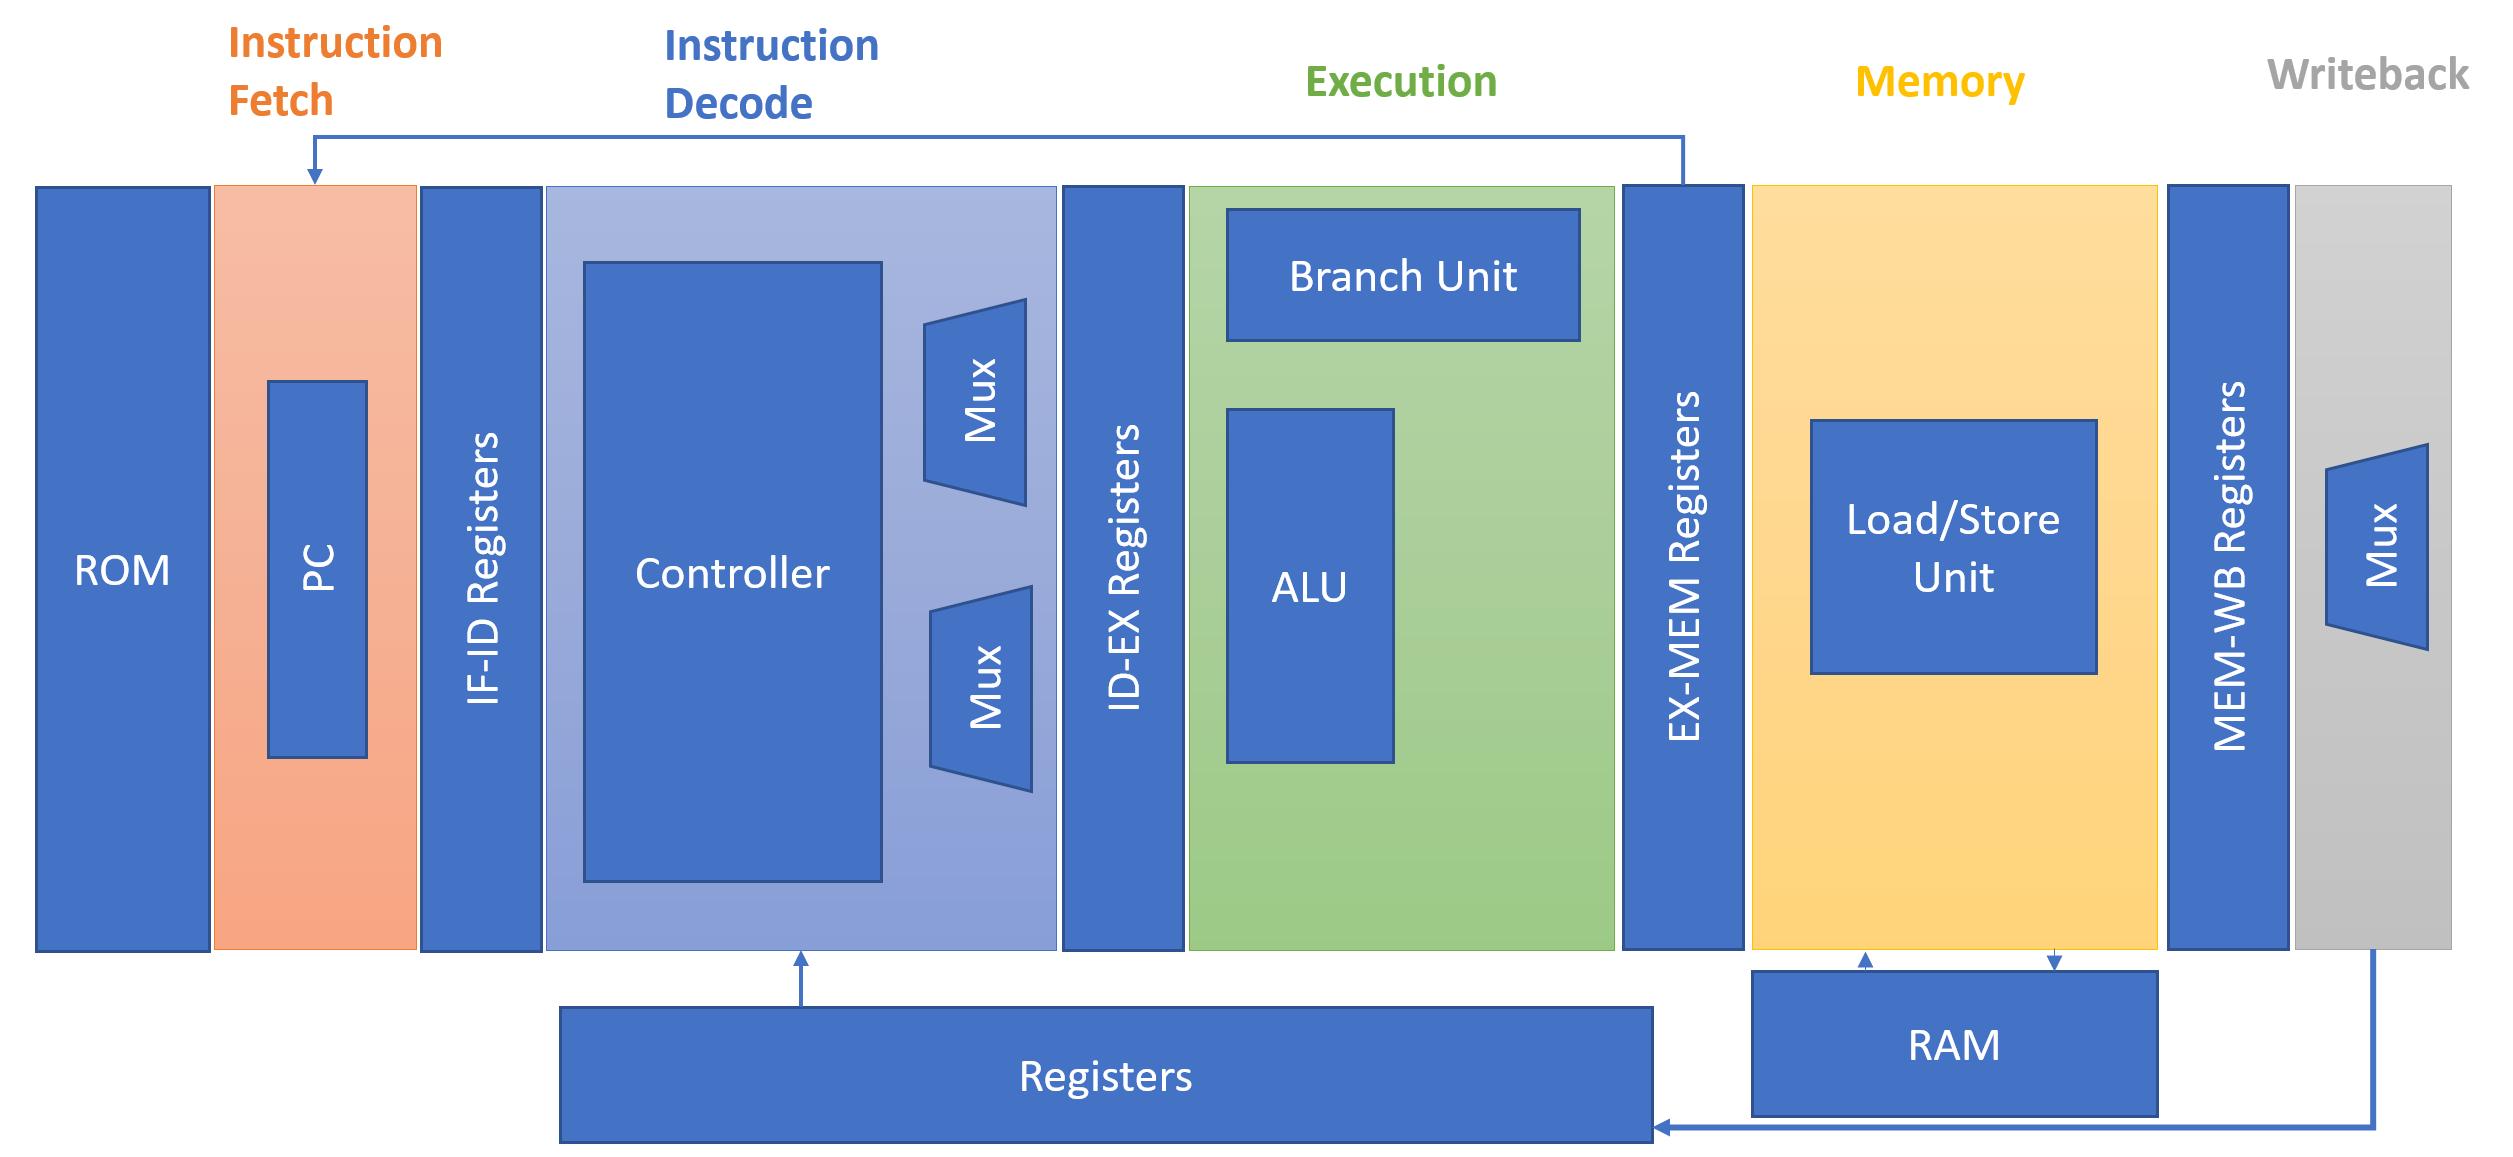
\includegraphics[width=1\textwidth]{design/pipelined/images/pipelined_design.png}
    \caption{Pipelined CPU design}
    \label{fig:pipelined_cpu_design}
\end{figure}

So here is the idea, we will divide the execution of instruction into five stages: Instruction Fetch (IF), Instruction Decode (ID), Execute (EX), Memory (MEM) and Write Back (WB).
Each stage will be executed in parallel and will be connected to the next one using pipeline registers. The pipeline registers are used to store the data between each stage and are synchronized with the clock.
The IF stage will fetch the instruction from the ROM using the PC (Program Counter) and will send it to the ID stage. The ID stage will decode the instruction and send the control signals to the different units 
(ALU, Branch Unit, Load/Store Unit) and will also send the operands to the EX stage. The EX stage will execute the instruction and send the result to the MEM stage. 
The MEM stage will load or store data from or to the RAM and send the result to the WB stage. Finally, the WB stage will write the result to the register file. \\

But for the most attentive reader or anybody with a bit of experience in computer architecture, you may have noticed that there is a problem with this design. 
This design will lead so some issues in two different ways. 

\begin{enumerate}[label=\textbullet]
    \item The first one is that since instruction is not executed anymore in one cycle, its result will not be available in the next cycle.
    This is an issue because if the next instruction depends on the result of the previous one, it will not be able to execute correctly and will use 
    outdated data from the registers. This is called a \textbf{Data Hazard}.
    \item The second one is related to the branching mechanism, since the result of the branch will be available only after the EX stage, the PC will not be updated
    before that leading to possible wrong instructions being fetched and executed in the pipeline. This is called a \textbf{Control Hazard}.
\end{enumerate}

For resolving these two issues we have two solutions. Either stalling the pipeline when a hazard is occurring or when a branch is detected at the IF stage such that we wait for 
the result before fetching any new instruction. One issue with this approach is of course performance which is unfortunate since the main purpose of pipelining is to improve performance.

Another solution for the data hazard is to use \textbf{Forwarding} which consists of forwarding the result of the ALU to the EX stage and the result of the MEM stage to the EX and MEM stages.
The only moment we will have to stall the pipeline is when we have a load instruction followed by an instruction using the result of the load. In this case, we will have to stall the pipeline
for one cycle to wait for the result of the load.

\begin{figure}[H]
    \centering
    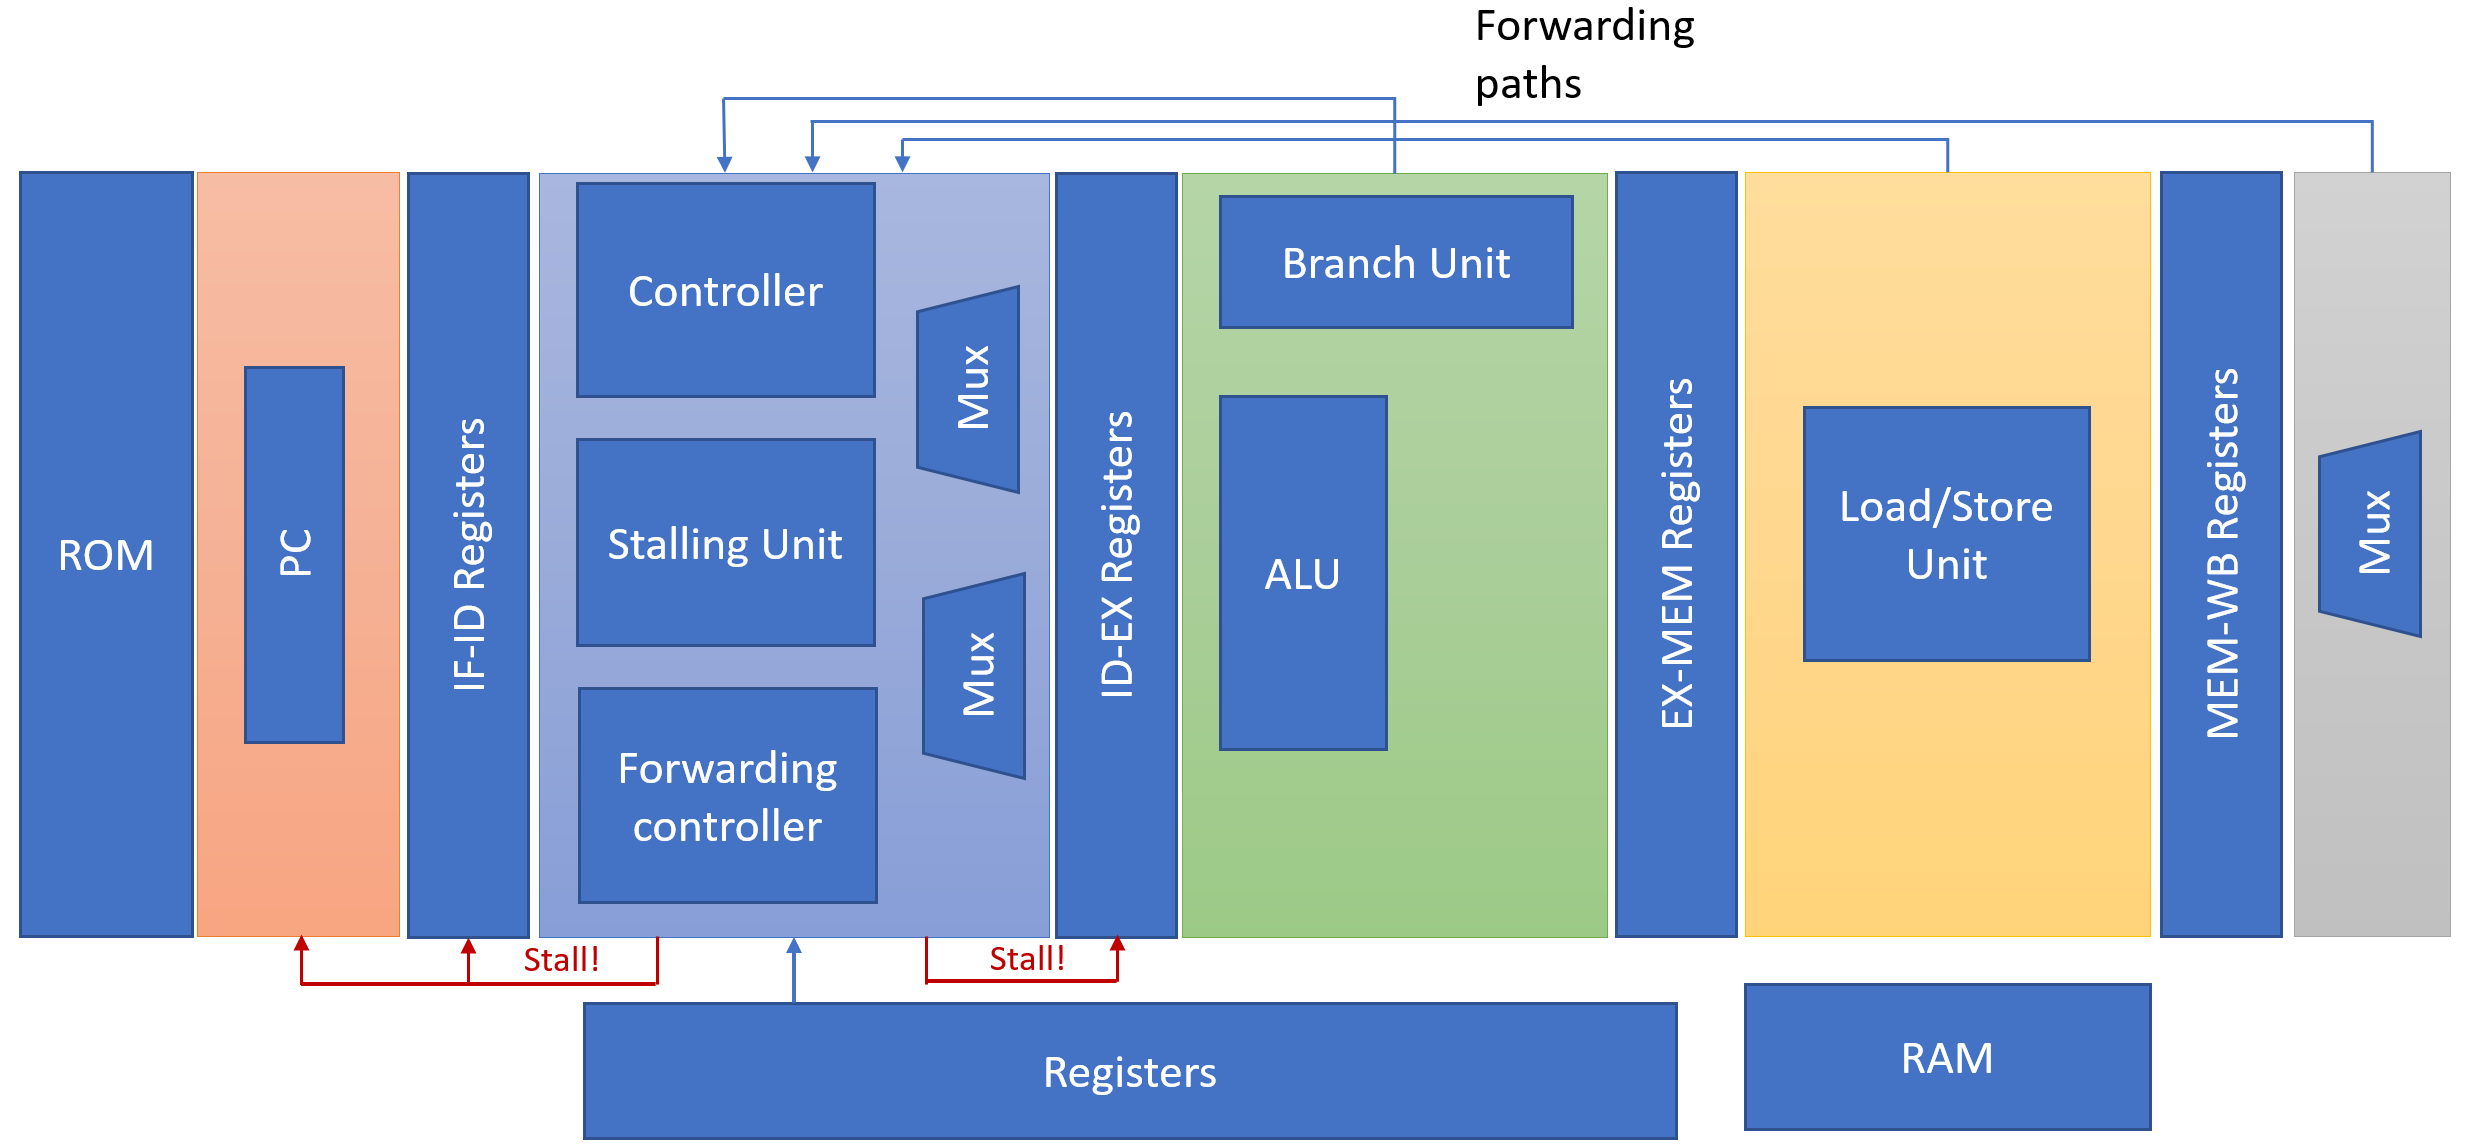
\includegraphics[width=1\textwidth]{design/pipelined/images/pipelined_design_forwarding.png}
    \caption{Pipelined CPU design with forwarding paths}
    \label{fig:pipelined_cpu_design_forwarding}
\end{figure}

Another solution for the control hazard is to use \textbf{Branch Prediction} which consists of predicting the result of the branch and fetching the instruction at the predicted address.
It is not always possible to predict correctly the result of a branch but it is possible to use some heuristics to improve the prediction accuracy. For example, we can predict that a branch will not be taken
if the previous branch was not taken. This is called a \textbf{Branch Not Taken} heuristic. Another heuristic is to predict that a branch will be taken if the previous branch was taken. This is called a \textbf{Branch Taken} heuristic.
Of course, you can develop more complex heuristics but this is out of the scope of this project and I invite you to use the link in the reference to the given algorithm I've chosen 
to implement in the CPU\@. But when the prediction is wrong, we will have to flush the pipeline and restart the execution from the correct address. \\

\begin{figure}[H]
    \centering
    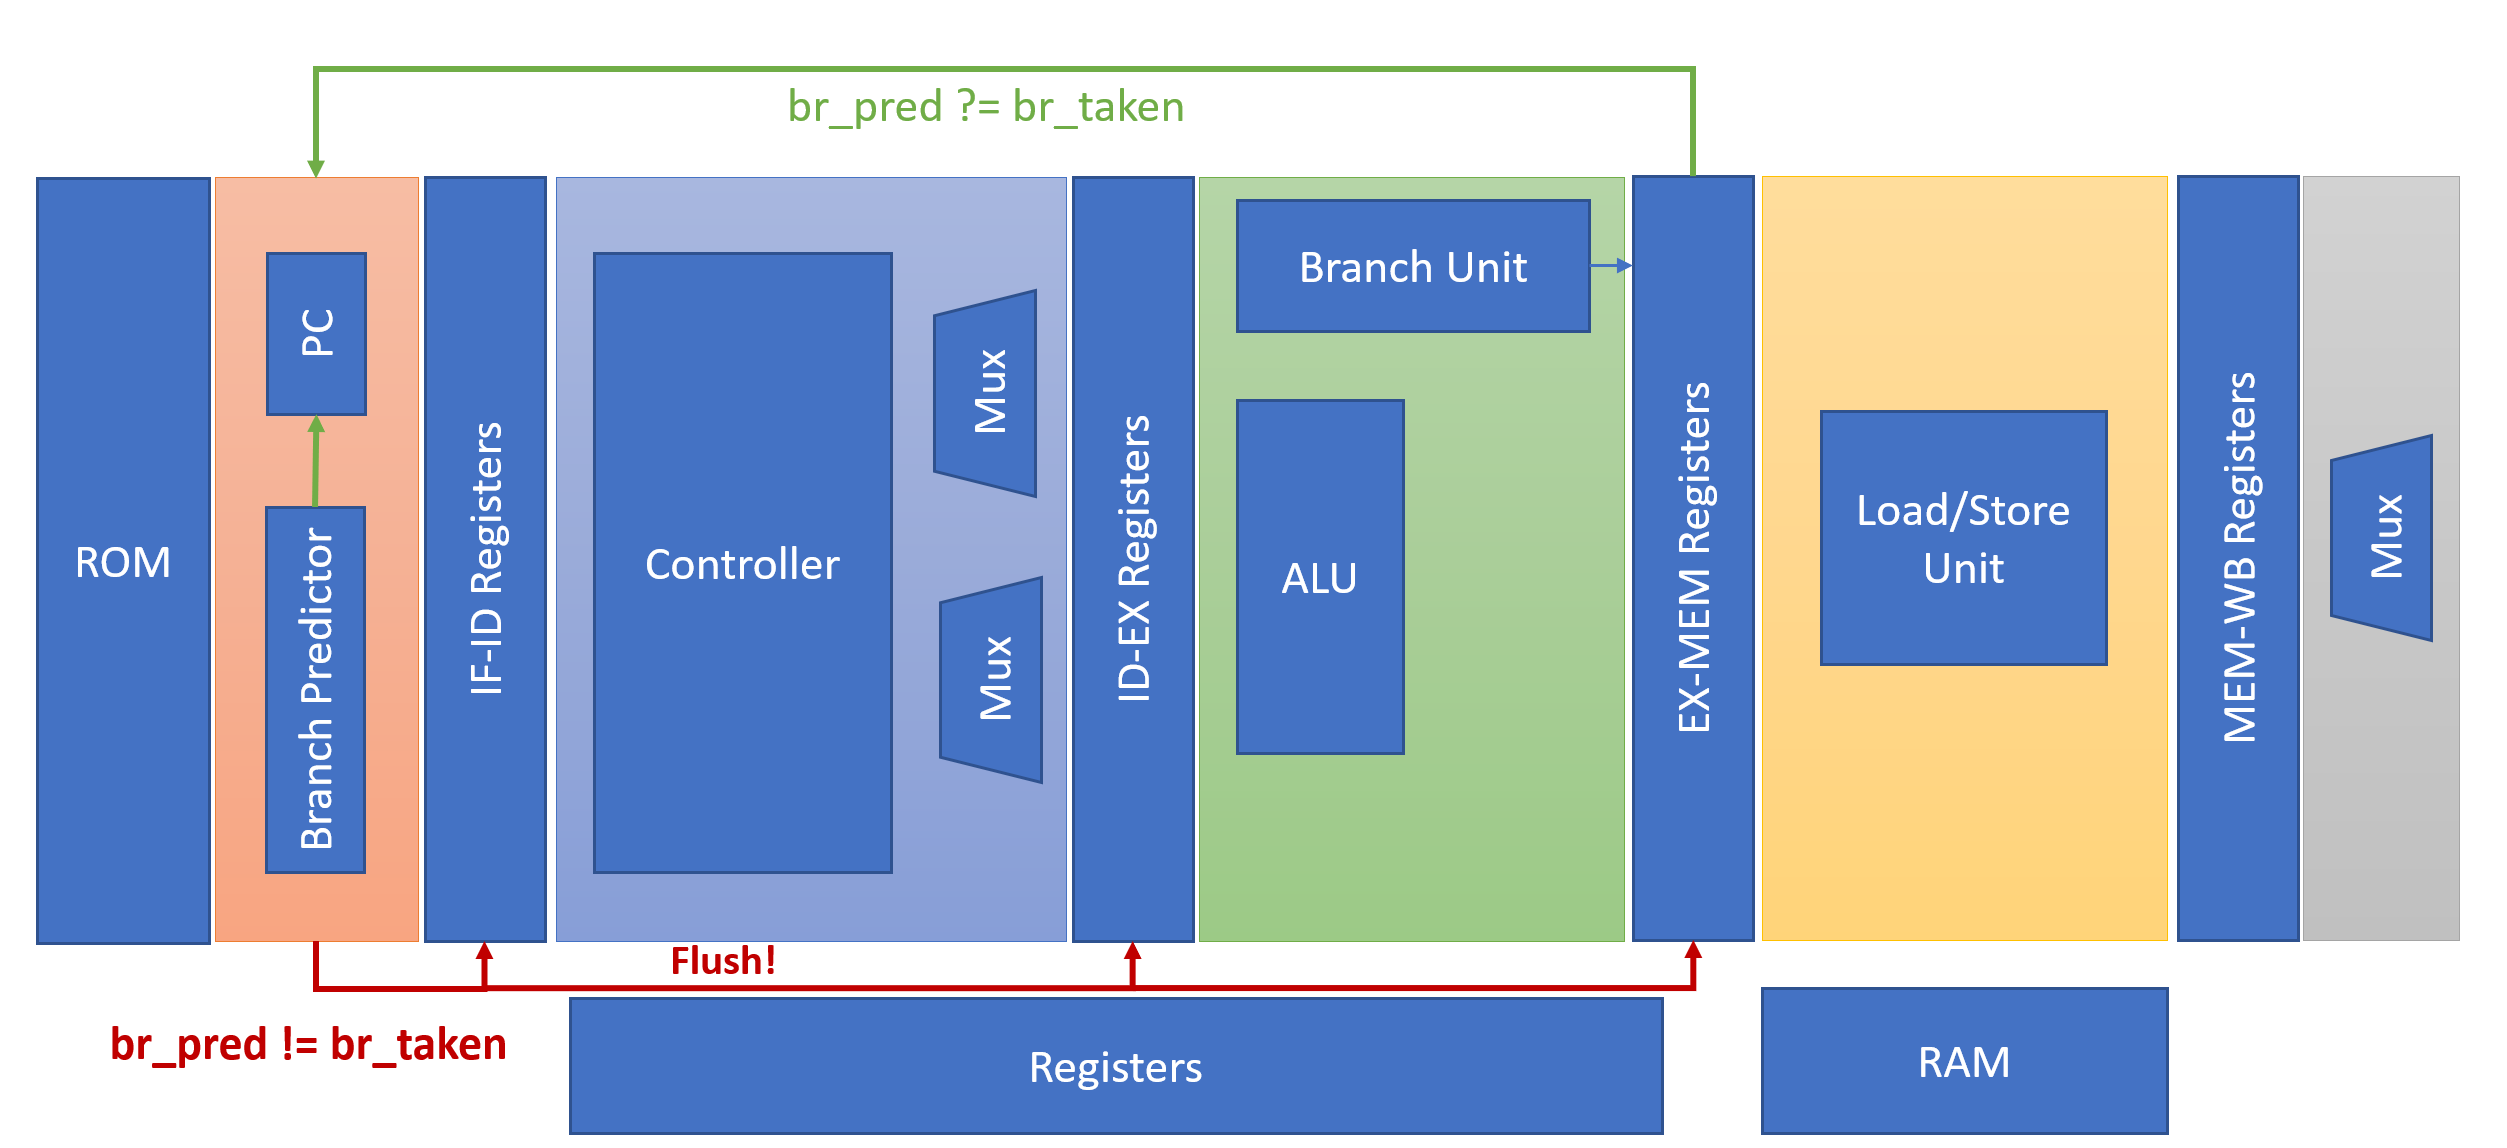
\includegraphics[width=1\textwidth]{design/pipelined/images/pipelined_design_predictor.png}
    \caption{Pipelined CPU design with branch predictor}
    \label{fig:pipelined_cpu_design_predictor}
\end{figure}



